\Case{open-0}{
\begin{tikzpicture}
  \draw plot[smooth] coordinates {};
\end{tikzpicture}}

\Case{open-1}{
\begin{tikzpicture}
  \draw plot[smooth] coordinates {(2pt,3pt)};
\end{tikzpicture}}

\Case{open-2}{
\begin{tikzpicture}
  \draw plot[smooth] coordinates {(2pt,3pt) (6pt,9pt)};
\end{tikzpicture}}

\Case{closed-0}{
\begin{tikzpicture}
  \draw plot[smooth cycle] coordinates {};
\end{tikzpicture}}

\Case{closed-1}{
\begin{tikzpicture}
  \draw plot[smooth cycle] coordinates {(2pt,3pt)};
\end{tikzpicture}}

\Case{closed-2}{
\begin{tikzpicture}
  \draw plot[smooth cycle] coordinates {(2pt,3pt) (6pt,9pt)};
\end{tikzpicture}}

\Case{open-join}{
\begin{tikzpicture}
  \draw (-8pt,-4pt) -- (-5pt,1pt) -- plot[smooth] coordinates
    {(2pt,3pt) (6pt,9pt) (10pt,4pt)} -- ++(1pt,2pt);
\end{tikzpicture}}

\Case{open-move}{
\begin{tikzpicture}
  \draw (-8pt,-4pt) -- (-5pt,1pt) plot[smooth] coordinates
    {(2pt,3pt) (6pt,9pt) (10pt,4pt)} -- ++(1pt,2pt);
\end{tikzpicture}}

\Case{closed-join}{
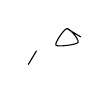
\begin{tikzpicture}
  \draw (-8pt,-4pt) -- (-5pt,1pt) -- plot[smooth cycle] coordinates
    {(2pt,3pt) (6pt,9pt) (10pt,4pt)} -- ++(1pt,2pt);
\end{tikzpicture}}

\Case{closed-move}{
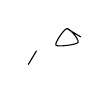
\begin{tikzpicture}
  \draw (-8pt,-4pt) -- (-5pt,1pt) plot[smooth cycle] coordinates
    {(2pt,3pt) (6pt,9pt) (10pt,4pt)} -- ++(1pt,2pt);
\end{tikzpicture}}

\Case{coincident-prefix}{
\begin{tikzpicture}
  \draw (2pt,3pt) -- plot[smooth] coordinates {(2pt,3pt) (6pt,9pt) (10pt,4pt)};
  \draw (2pt,3pt) plot[smooth] coordinates {(2pt,3pt) (6pt,9pt) (10pt,4pt)};
\end{tikzpicture}}

\Case{relative-samples}{
\begin{tikzpicture}
  \draw (20pt,30pt) -- plot[smooth] coordinates
    {(2pt,3pt) +(4pt,5pt) ++(6pt,7pt) +(8pt,9pt)}
    -- +(1pt,2pt) -- ++(3pt,4pt);
\end{tikzpicture}}

\Case{empty-continued}{
\begin{tikzpicture}
  \draw (20pt,30pt) -- (8pt,9pt) -- plot[smooth] coordinates {} -- ++(1pt,2pt);
  \draw (20pt,30pt) -- (8pt,9pt) plot[smooth cycle] coordinates {} -- ++(1pt,2pt);
\end{tikzpicture}}

\Case{one-continued}{
\begin{tikzpicture}
  \draw (20pt,30pt) -- plot[smooth] coordinates {(2pt,3pt)} -- ++(1pt,2pt);
  \draw (20pt,30pt) -- plot[smooth cycle] coordinates {(2pt,3pt)} -- ++(1pt,2pt);
\end{tikzpicture}}

\Case{two-continued}{
\begin{tikzpicture}
  \draw (20pt,30pt) -- plot[smooth] coordinates {(2pt,3pt) (6pt,9pt)} -- ++(1pt,2pt);
  \draw (20pt,30pt) -- plot[smooth cycle] coordinates {(2pt,3pt) (6pt,9pt)} -- ++(1pt,2pt);
\end{tikzpicture}}

\Case{relative-move-after-plot}{
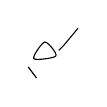
\begin{tikzpicture}
  \draw (20pt,30pt) -- +(3pt,-4pt) -- plot[smooth cycle] coordinates
    {+(2pt,3pt) ++(6pt,9pt) +(10pt,4pt)}
    +(1pt,2pt) -- ++(3pt,4pt) -- +(5pt,6pt);
\end{tikzpicture}}

\Case{close-after-join}{
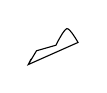
\begin{tikzpicture}
  \draw (-8pt,-4pt) -- (-5pt,1pt) -- plot[smooth] coordinates
    {(2pt,3pt) (6pt,9pt) (10pt,4pt)} -- cycle -- ++(1pt,2pt);
\end{tikzpicture}}

\Case{close-after-move}{
\begin{tikzpicture}
  \draw (-8pt,-4pt) -- (-5pt,1pt) plot[smooth] coordinates
    {(2pt,3pt) (6pt,9pt) (10pt,4pt)} -- cycle -- ++(1pt,2pt);
\end{tikzpicture}}

\Case{duplicate-neighbours}{
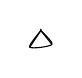
\begin{tikzpicture}
  \draw plot[smooth] coordinates {(2pt,3pt) (6pt,9pt) (6pt,9pt) (10pt,4pt)};
  \draw plot[smooth cycle] coordinates {(2pt,3pt) (6pt,9pt) (6pt,9pt) (10pt,4pt)};
\end{tikzpicture}}

\Case{repeated-closing-point}{
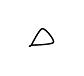
\begin{tikzpicture}
  \draw plot[smooth] coordinates {(2pt,3pt) (6pt,9pt) (10pt,4pt) (2pt,3pt)};
  \draw plot[smooth cycle] coordinates {(2pt,3pt) (6pt,9pt) (10pt,4pt) (2pt,3pt)};
\end{tikzpicture}}

\Case{coincident-samples}{
\begin{tikzpicture}
  \draw plot[smooth] coordinates {(6pt,9pt) (6pt,9pt) (6pt,9pt)};
  \draw plot[smooth cycle] coordinates {(6pt,9pt) (6pt,9pt) (6pt,9pt)};
\end{tikzpicture}}

\Case{tension-zero}{
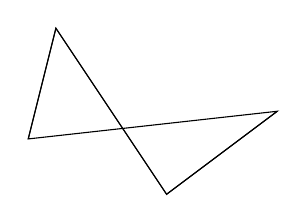
\begin{tikzpicture}
  \draw plot[smooth,tension=0] coordinates {(0pt,0pt) (10pt,40pt) (50pt,-20pt) (90pt,10pt)};
  \draw plot[smooth cycle,tension=0] coordinates {(0pt,0pt) (10pt,40pt) (50pt,-20pt) (90pt,10pt)};
\end{tikzpicture}}

\Case{tension-negative}{
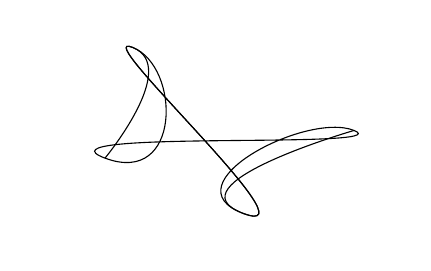
\begin{tikzpicture}
  \draw plot[smooth,tension=-1.25] coordinates {(0pt,0pt) (10pt,40pt) (50pt,-20pt) (90pt,10pt)};
  \draw plot[smooth cycle,tension=-1.25] coordinates {(0pt,0pt) (10pt,40pt) (50pt,-20pt) (90pt,10pt)};
\end{tikzpicture}}

\Case{tension-large-open}{
\begin{tikzpicture}
  \draw[line width=2pt] plot[smooth,tension=6] coordinates
    {(0pt,0pt) (10pt,40pt) (50pt,-20pt) (90pt,10pt)};
\end{tikzpicture}}

\Case{tension-large-closed}{
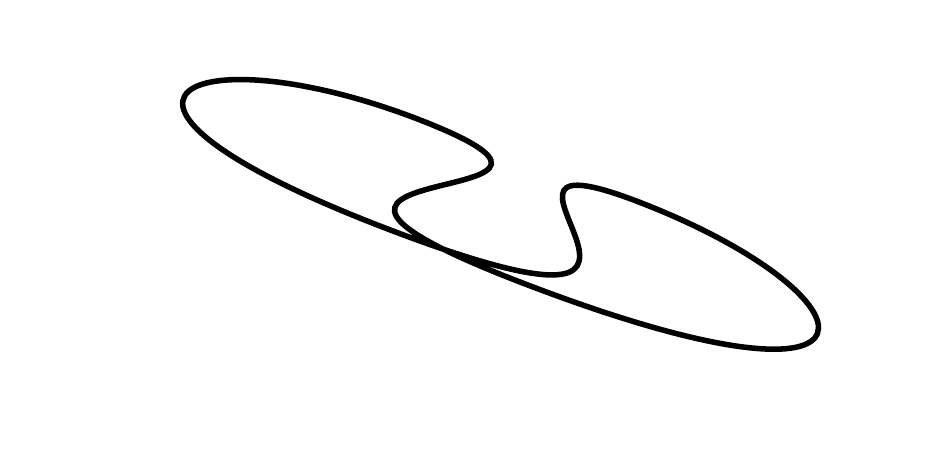
\begin{tikzpicture}
  \draw[line width=2pt] plot[smooth cycle,tension=6] coordinates
    {(0pt,0pt) (10pt,40pt) (50pt,-20pt) (90pt,10pt)};
\end{tikzpicture}}

\Case{scope-restoration}{
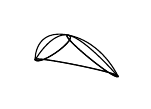
\begin{tikzpicture}[smooth,tension=.75]
  \begin{scope}[smooth cycle,tension=-.5]
    \draw plot coordinates {(0pt,0pt) (12pt,9pt) (30pt,-6pt)};
    \draw[smooth,tension=1.5] plot coordinates {(0pt,0pt) (12pt,9pt) (30pt,-6pt)};
    \draw plot coordinates {(0pt,0pt) (12pt,9pt) (30pt,-6pt)};
  \end{scope}
  \draw plot coordinates {(0pt,0pt) (12pt,9pt) (30pt,-6pt)};
\end{tikzpicture}}

\Case{adjacent-plot-options}{
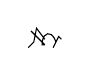
\begin{tikzpicture}
  \draw[smooth,tension=1.5] (1pt,2pt)
    -- plot[tension=0] coordinates {(3pt,4pt) (4pt,9pt) (7pt,5pt)}
    plot[smooth cycle,tension=-1] coordinates {(2pt,8pt) (7pt,3pt) (4pt,6pt)}
    -- plot coordinates {(6pt,3pt) (8pt,7pt) (11pt,4pt)}
    plot[sharp plot] coordinates {(10pt,2pt) (12pt,6pt) (13pt,5pt)};
\end{tikzpicture}}

\Case{every-plot}{
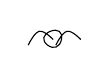
\begin{tikzpicture}[every plot/.style={smooth,tension=.75}]
  \draw plot coordinates {(1pt,1pt) (5pt,6pt) (10pt,3pt)}
    -- plot[smooth cycle,tension=2] coordinates {(8pt,1pt) (9pt,6pt) (13pt,3pt)}
    plot coordinates {(11pt,1pt) (15pt,6pt) (20pt,3pt)};
\end{tikzpicture}}

\Case{transformed-explicit}{
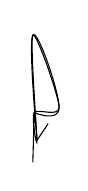
\begin{tikzpicture}[x={(8pt,3pt)},y={(-2pt,5pt)},shift={(12pt,-7pt)},rotate=90]
  \draw[yscale=-.5] (-1,1) -- plot[smooth,tension=.75] coordinates
    {(1,0) (2,3) (4,-2) (0,1)} -- ++(1,1);
  \draw[yscale=-.5] plot[smooth cycle] coordinates {(1,0) (2,3) (4,-2) (0,1)};
\end{tikzpicture}}

\Case{plot-local-transform}{
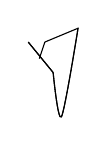
\begin{tikzpicture}[x=2pt,y=3pt]
  \draw (4pt,3pt) -- plot[smooth,x=3pt,y=4pt,xshift=10pt,yscale=-2] coordinates
    {(1,1) (2,3) (4,-1)} -- ++(1,2);
  \draw (4pt,3pt) -- plot[smooth,x=3pt,y=4pt,xshift=10pt,yscale=-2] coordinates
    {(1,1) (2,3) (4,-1)} +(0pt,0pt) -- ++(1,2);
\end{tikzpicture}}

\Case{parametric-open}{
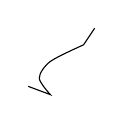
\begin{tikzpicture}[x=4pt,y=3pt,xshift=-7pt]
  \draw (-2,0) -- plot[smooth,variable=\t,domain=-1:2,samples=4]
    ({\t*\t-1},{2*\t+1}) -- ++(1,2);
\end{tikzpicture}}

\Case{explicit-open}{
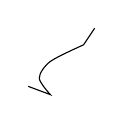
\begin{tikzpicture}[x=4pt,y=3pt,xshift=-7pt]
  \draw (-2,0) -- plot[smooth] coordinates {(0,-1) (-1,1) (0,3) (3,5)} -- ++(1,2);
\end{tikzpicture}}

\Case{parametric-closed}{
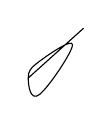
\begin{tikzpicture}[x=4pt,y=3pt,xshift=-7pt]
  \draw plot[smooth cycle,tension=.75,variable=\t,domain=-1:2,samples=4]
    ({\t*\t-1},{2*\t+1}) -- ++(1,2);
\end{tikzpicture}}

\Case{nonuniform-parametric}{
\begin{tikzpicture}[x=4pt,y=3pt]
  \draw plot[smooth,tension=1,variable=\t,samples at={0,.25,1.5,2}]
    ({2*\t},{\t*\t});
\end{tikzpicture}}

\Case{ordinary-plot}{
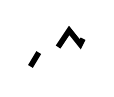
\begin{tikzpicture}
  \draw[line width=2pt] (-8pt,-4pt) -- (-5pt,1pt) plot coordinates
    {(2pt,3pt) (6pt,9pt) (10pt,4pt)} -- (11pt,6pt);
\end{tikzpicture}}

\Case{ordinary-cubic}{
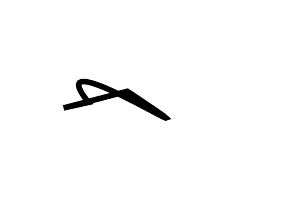
\begin{tikzpicture}
  \draw[line width=2pt] (-8pt,2pt) -- (1pt,4pt)
    .. controls (-20pt,30pt) and (60pt,-22pt) .. (15pt,8pt) -- cycle;
\end{tikzpicture}}

\Case{legacy-tension-one}{
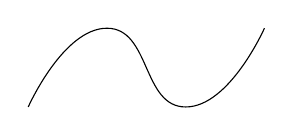
\begin{tikzpicture}
  \draw plot [smooth, tension=1] coordinates { (0,0) (1,1) (2,0) (3,1) };
\end{tikzpicture}}
